\section{Experiment 10A: nonlinear basis-order and coverage audit}
\label{sec:experiment10a}

\paragraph{Why this experiment is necessary.}
The earlier cold-start study identifies only three positive physical ratios.
That model extrapolates unusually well from short local recordings because its
speed dependence is imposed analytically. Restricting the amount of data alone
therefore does not create a defensible need for cross-client information. The
new experiment sequence asks a narrower question: can complementary client
coverage help identify a richer LPV map that is genuinely required by nonlinear
lateral dynamics?

Experiment 10A is a representation and identifiability gate before any new FL
comparison. It must establish three facts. First, the frozen physics basis must
remain sufficient where the plant is effectively linear. Second, nonlinear
operating points must justify additional speed dependence under validation on
entirely withheld speed regions. Third, a client restricted to one part of the
speed envelope may be locally underdetermined while the union of complementary
clients is identifiable. Failure of either of the last two conditions stops the
planned Experiment 10B.

\paragraph{Operating-point construction.}
The data-generating plant is the existing nonlinear tanh-tire bicycle model;
10A does not introduce an artificial high-order plant. For speed $v$ and road
curvature $\kappa$, the steady-cornering point satisfies
\begin{equation}
 r^\star=v\kappa,\qquad
 f_{\mathrm{nl}}\!\left([\beta^\star,r^\star]^\top,
 \delta^\star,v\right)=0.
\end{equation}
The continuous Jacobians with respect to state and steering are evaluated by
centered finite differences and discretized exactly under zero-order hold at
$T_s=0.01$~s. This gives speed-indexed local models along physically meaningful
turning equilibria rather than only around straight-line motion. The audit uses
$\kappa\in\{0,0.0025,0.005\}\,\mathrm{m}^{-1}$ and
$v\in\{10,12,\ldots,30\}\,\mathrm{m\,s}^{-1}$. The most severe point has
$a_y=v^2\kappa=4.5\,\mathrm{m\,s}^{-2}$; across all clients, the equilibrium
range remains within $|\beta^\star|\leq2.37^\circ$ and
$|\delta^\star|\leq2.27^\circ$.

\paragraph{Nested basis family and selection rule.}
The baseline order is the previously validated physics basis
\begin{equation}
 \Phi_3(v)=[1,v^{-1},v^{-2}].
\end{equation}
Orders $L=4,\ldots,7$ append the nested normalized-speed terms
$z,z^2,z^3,z^4$, where $z=(v-20)/10$. Thus each candidate is a Laurent
polynomial that retains the known reciprocal physics while adding smooth
residual freedom. To avoid the severe collinearity of raw reciprocal and
polynomial columns, each candidate space is transformed by QR orthogonalization
on a fixed 401-point grid over $10$--$30\,\mathrm{m\,s}^{-1}$. This is an
invertible change of coordinates: it improves numerical conditioning without
changing the functions contained in a candidate space. It also avoids an
arbitrary ordering of hand-placed radial-basis centers.

Five cross-validation folds withhold contiguous speed regions:
$\{10,12\}$, $\{14,16\}$, $\{18,20,22\}$, $\{24,26\}$, and $\{28,30\}$.
This is deliberately harder than random sample splitting because no neighboring
sample at the same withheld speed is available. The score is relative Frobenius
error of the stacked $[A_d,B_d]$ entries. It is first averaged over clients and
folds within each independent fleet. The chosen order is the smallest order
within one fleet-level standard error of the best mean, subject to conditioning.
Errors below $10^{-4}$ relative, or $0.01\%$, are treated as practically
equivalent. This floor prevents numerical differences in an already exact model
from rewarding unnecessary basis terms.

The development population comprises 300 vehicles from ten independent fleet
seeds. In total, 22500 blocked validation fits are evaluated. No controller
tracking result or later test fleet enters the order selection.

\begin{table}[htbp]
\centering
\caption{Experiment 10A blocked-speed matrix error. Entries are percentages;
``worst'' is the largest client--fold error over all development fleets.}
\label{tab:experiment10a-basis}
\begin{tabular}{rrrrrr}
\toprule
$\kappa$ [m$^{-1}$] & $L$ & Mean & Fleet SE & Worst & $\kappa_2$ worst\\
\midrule
0       & 3 & 0.0008 & $4.89\!\times\!10^{-6}$ & 0.0044 & 27.47\\
0       & 7 & 0.00004 & $2.50\!\times\!10^{-7}$ & 0.0003 & 240.38\\
0.0025  & 3 & 0.6604 & 0.0011 & 2.3584 & 27.47\\
0.0025  & 6 & 0.0047 & $8.69\!\times\!10^{-6}$ & 0.0230 & 68.95\\
0.0025  & 7 & 0.00006 & $3.04\!\times\!10^{-7}$ & 0.0004 & 240.38\\
0.0050  & 3 & 2.6607 & 0.0044 & 9.5054 & 27.47\\
0.0050  & 4 & 0.9669 & 0.0016 & 4.1013 & 28.46\\
0.0050  & 5 & 0.2081 & 0.0004 & 0.9593 & 32.24\\
0.0050  & 6 & 0.0210 & 0.00004 & 0.1048 & 68.95\\
0.0050  & 7 & 0.0007 & $3.59\!\times\!10^{-6}$ & 0.0047 & 240.38\\
\bottomrule
\end{tabular}
\end{table}

\begin{figure}[htbp]
\centering
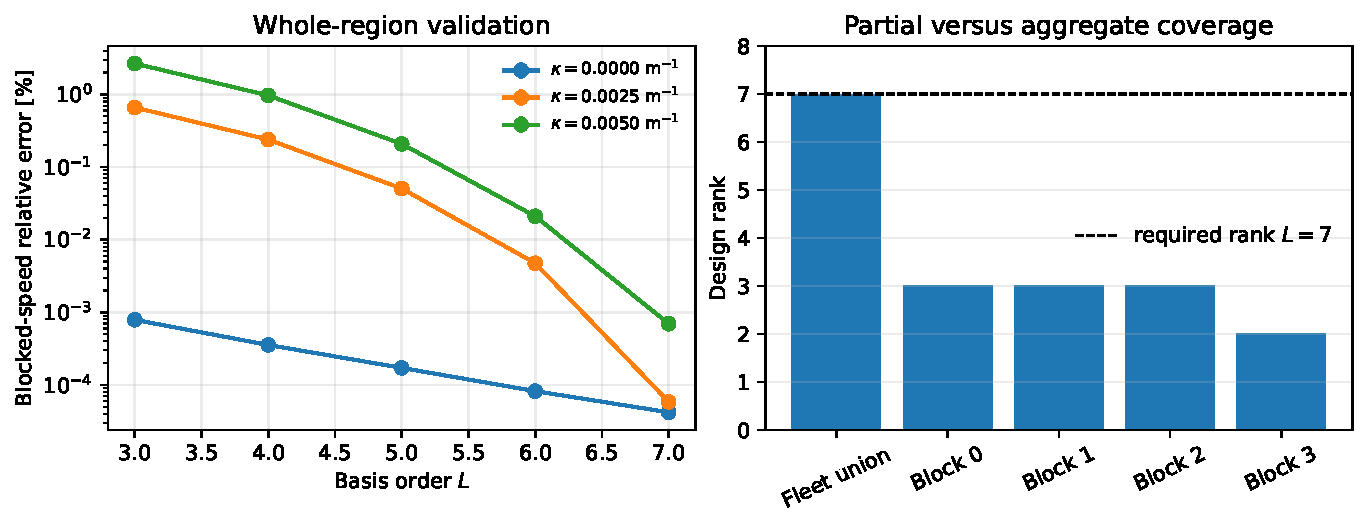
\includegraphics[width=0.95\linewidth]{../results/figures/experiment_10a_basis_coverage_audit.pdf}
\caption{Blocked-speed basis audit and design-rank comparison. The nonlinear
cornering cases require residual speed dependence, while no restricted local
block can identify the seven selected coefficients.}
\label{fig:experiment10a}
\end{figure}

\paragraph{Results.}
The straight-line negative control behaves as required. All candidate bases are
already far below the practical error floor, so the rule retains $L=3$ despite
the numerically smallest value occurring at $L=7$. Extra flexibility is not
justified for the original small-signal model.

The nonlinear operating points require more structure. At
$\kappa=0.0025\,\mathrm{m}^{-1}$, $L=6$ is the smallest model below the
$0.01\%$ practical floor; its mean blocked-speed error is $0.0047\%$, compared
with $0.6604\%$ for $L=3$. At $\kappa=0.005\,\mathrm{m}^{-1}$, the rule selects
$L=7$. Mean error falls monotonically from $2.6607\%$ at $L=3$ to $0.0007\%$
at $L=7$, and the worst client--fold error falls from $9.51\%$ to $0.0047\%$.
The strongest audited operating condition therefore determines the common
order $L=7$. The orthogonalized blocked-training condition number remains below
241, so this conclusion is not purchased by numerically singular regression.

\paragraph{Partial-coverage rank audit.}
For the selected $L=7$ model, a client assigned to one of the four speed blocks
$\{10,12,14\}$, $\{16,18,20\}$, $\{22,24,26\}$, or $\{28,30\}$ has design
rank three, three, three, or two, respectively. Every local block is therefore
rank deficient. The union of the eleven fleet speeds has rank seven and a
condition number of 3.41 in the fixed orthogonalized coordinates; the worst
blocked-training condition number across validation folds is 240.38.
Thus complementary coverage supplies structurally missing scheduling
information rather than merely more repetitions of the same local experiment.

\paragraph{Decision and limitation.}
Experiment 10A passes its representation and identifiability gate and freezes
\begin{equation}
 \boxed{L=7,\quad
 \operatorname{span}\Phi_7(v)=
 \operatorname{span}[1,v^{-1},v^{-2},z,z^2,z^3,z^4],\quad
 z=(v-20)/10.}
\end{equation}
This conclusion is narrower than an FL benefit. The targets are exact local
Jacobians, the operating points use known curvature, and rank deficiency alone
does not prove improved estimation or closed-loop control. Experiment 10B must
fit the frozen model from noisy complementary recordings and compare Local,
pooled compatible sharing, and an equal-budget local-information oracle on
unseen speeds. If sharing does not improve those outcomes, the new direction
must again be rejected or reframed.

\paragraph{Reproducibility.}
The frozen protocol, implementation, aggregate tables, client--fold records,
operating points, coverage diagnostics, and provenance hashes are stored in
\path{code/config/experiment_10a.json},
\path{code/experiments/experiment_10a_basis_coverage_audit.py}, and
\path{results/tables}.
